% !TeX encoding = UTF-8
% !TeX program = xelatex
% !TeX spellcheck = fr
\documentclass[10pt,a4paper]{report}

\usepackage[informatique]{styles/preambule_college}
\usepackage{styles/preambule_personnalisation}


\title{Fiches pratiques}
\author{S. Vannay}
\date{12.09.2022}

\begin{document}





\chapterFormat
\chapter*{Figures 2D de GeoGebra à TikZ}





\section{Workflow et fichiers utilisés}

\begin{enumerate}
	\item Le dessin de la figure se fait en GeoGebra dans le répertoire \incmd{figures_src}. Par exemple dans le fichier \incmd{figures_src/fig_01_01_diag_cartesien.ggb}.
	\item La figure est exportée au format TikZ avec le menu
		\begin{center}
			Fichier \textrightarrow \ Exporter \textrightarrow \ Graphique vers PGF/TikZ ... 
		\end{center}
		Un fichier \incmd{.tex} est créé dans le même répertoire. Avec l'exemple précédent, le fichier créé s'appelle \newline 
		\incmd{figures_src/fig_01_01_diag_cartesien.tex}
	\item On modifie le code TikZ dans le fichier \incmd{.tex} pour mettre au point la figure.
	\item Lorsque la figure est prête, on copie-colle l'environnement \incmd{tikzpicture} dans un fichier \incmd{.tikz} dans le répertoire \incmd{figures}, par exemple \incmd{figures/fig_01_01_diag_cartesien.tikz}
	\item Dans le document principal, on importe le \incmd{.tikz} :
		\begin{center}
			\inlatex{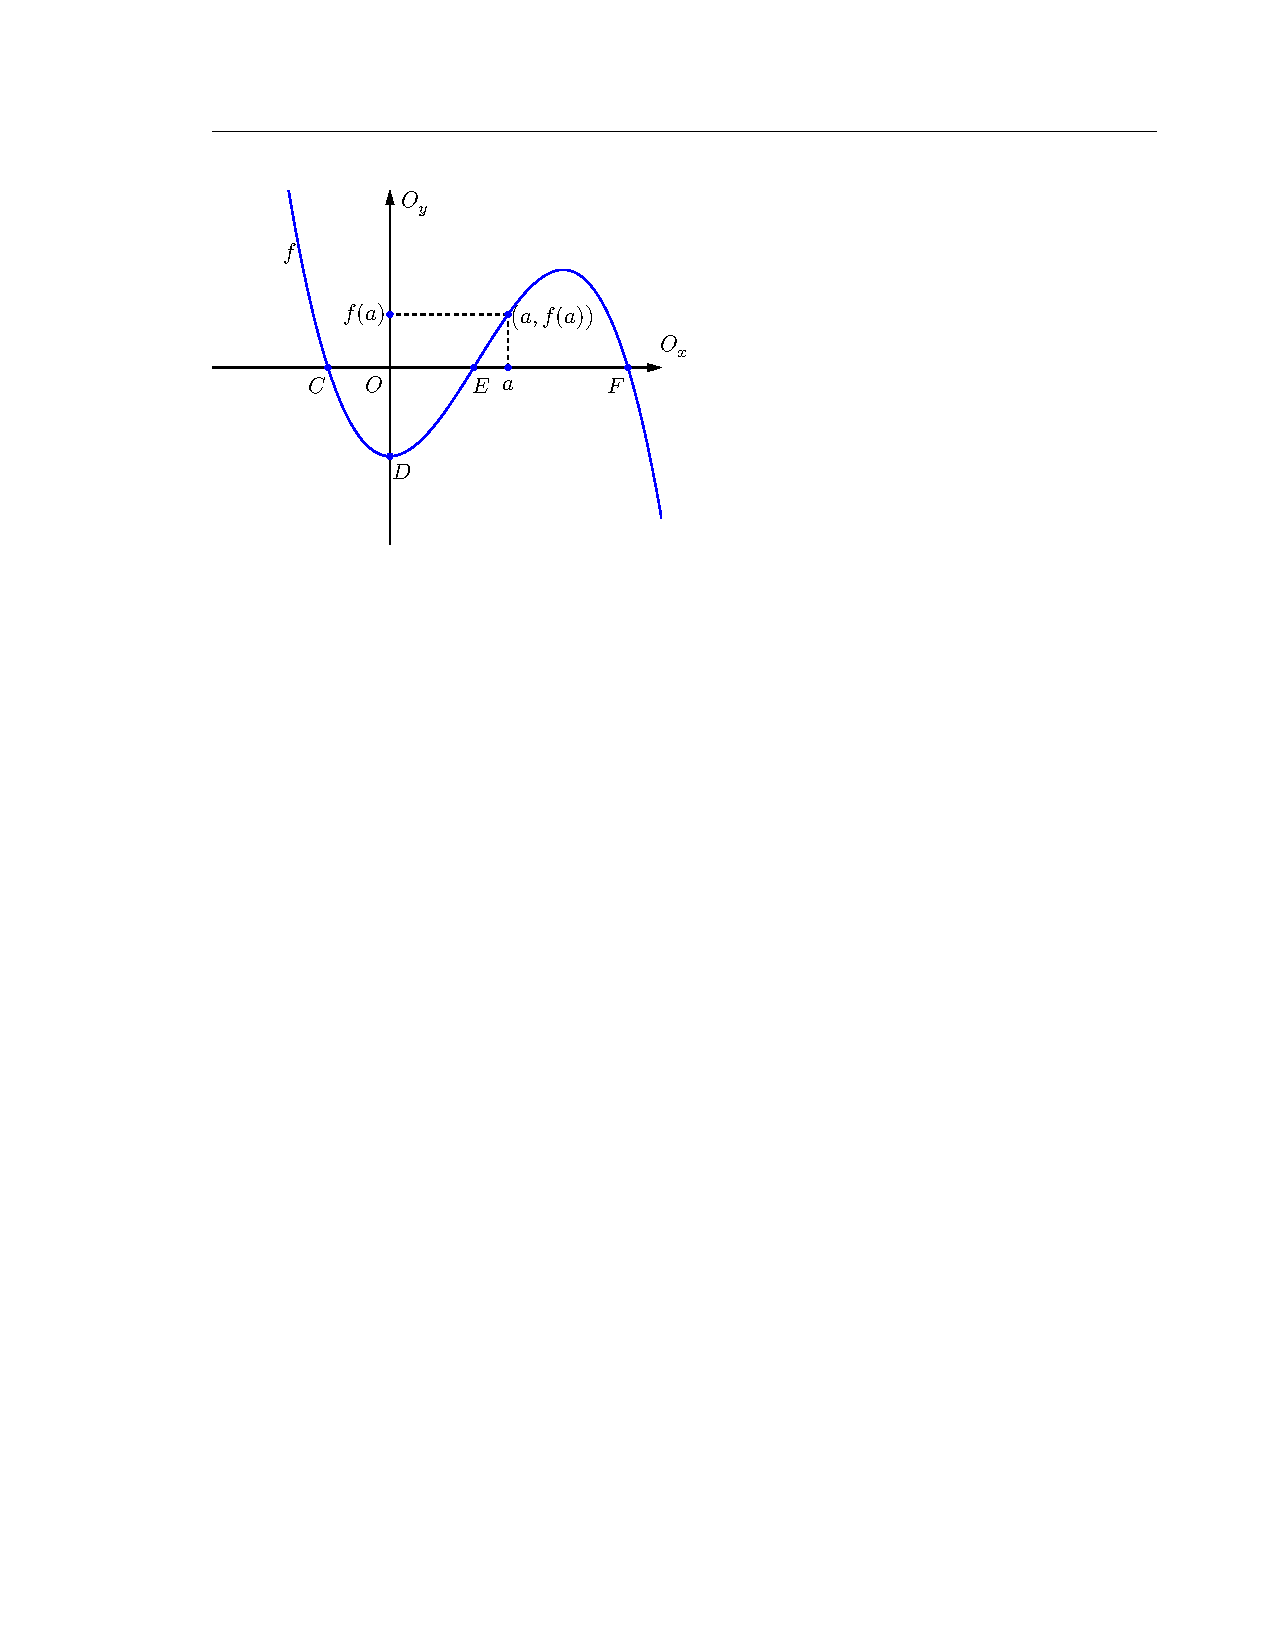
\includegraphics{figures/fig_01_01_diag_cartesien.tikz}}
		\end{center}
\end{enumerate}





\section{Paramétrage de GeoGebra}

Les figures 2D sont faites sur le modèle de la figure \incmd{fig_01_01_diag_cartesien.ggb}. Lorsqu'on l'ouvre avec GeoGebra 5 ou GeoGebra Classic, il faut vérifier les points suivants.



\subsection{La vue "Algèbre" est activée}

\begin{minipage}{.48\linewidth}
	\begin{figure}[H]
		\centering
		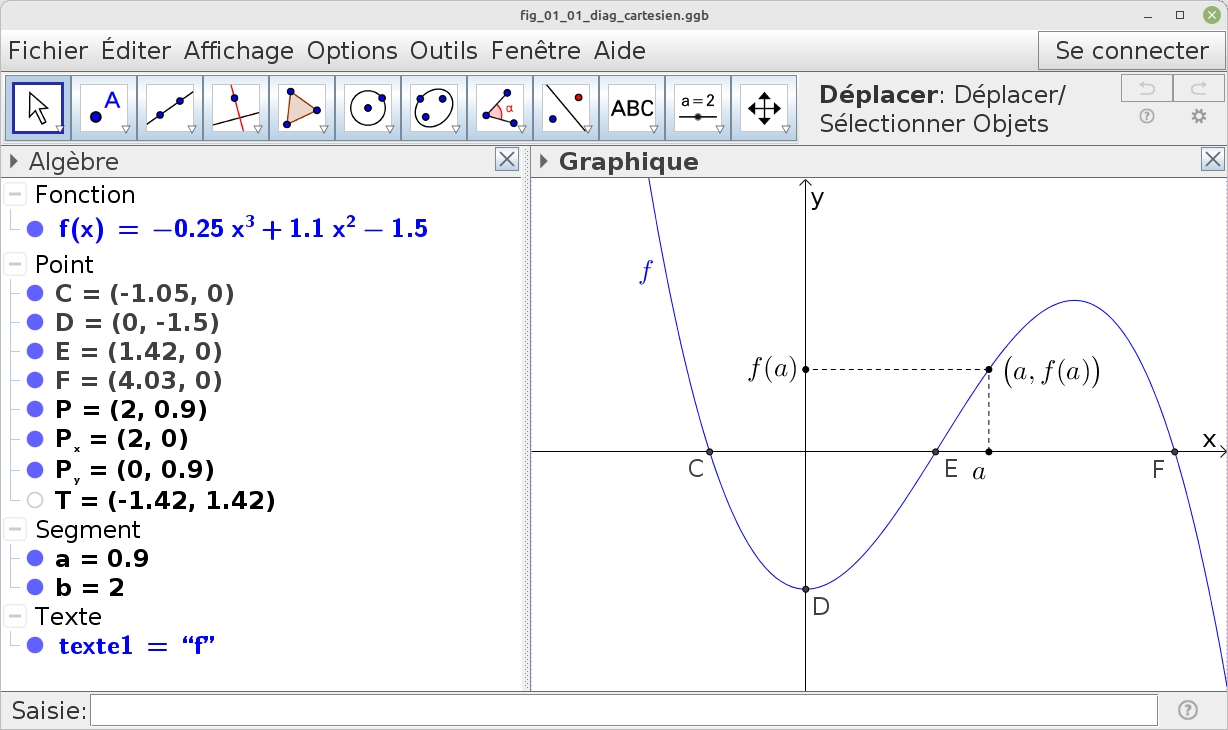
\includegraphics[width=\linewidth]{captures/interface_geogebra}
		\caption{}
		\label{fig:interface_geogebra}
	\end{figure}
\end{minipage}
\hfill
\begin{minipage}{.48\linewidth}
	\begin{figure}[H]
		\centering
		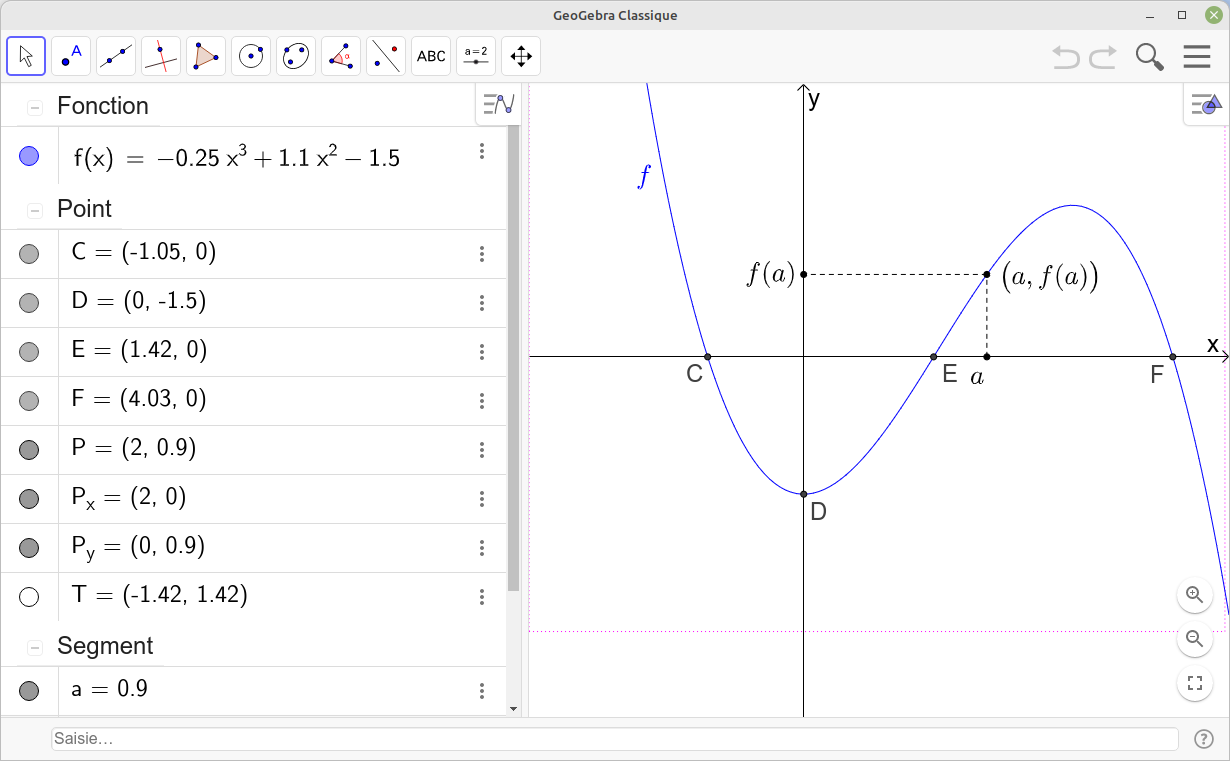
\includegraphics[width=\linewidth]{captures/interface_geogebra_classic}
		\caption{}
		\label{fig:interface_geogebra_classic}
	\end{figure}
\end{minipage}



\subsection{La taille d'affichage}

\vspace*{-3ex}
\begin{center}
	\item Menu \incmd{Option} \textrightarrow \ \incmd{Taille des caractères}
\end{center}

Problème : la taille d'affichage modifier la fonte du graphique mais aussi la fonte de l'interface.

Réglage :
\begin{enumerate}
	\item au moins 24 points pour que ce soit lisible par les étudiants si on veut projeter la figure en classe (mais l'interface devient pénible sur un écran de faible résolution);
	\item aussi petit qu'on veut si on ne prévoit pas de présenter la figure\dots
\end{enumerate}



\subsection{Les objets auxiliaires sont affichés}

Les objets auxiliaires définissent le cadre \incmd{ExpCadre} qui sera finalement exporté.

\begin{figure}[H]
	\centering
	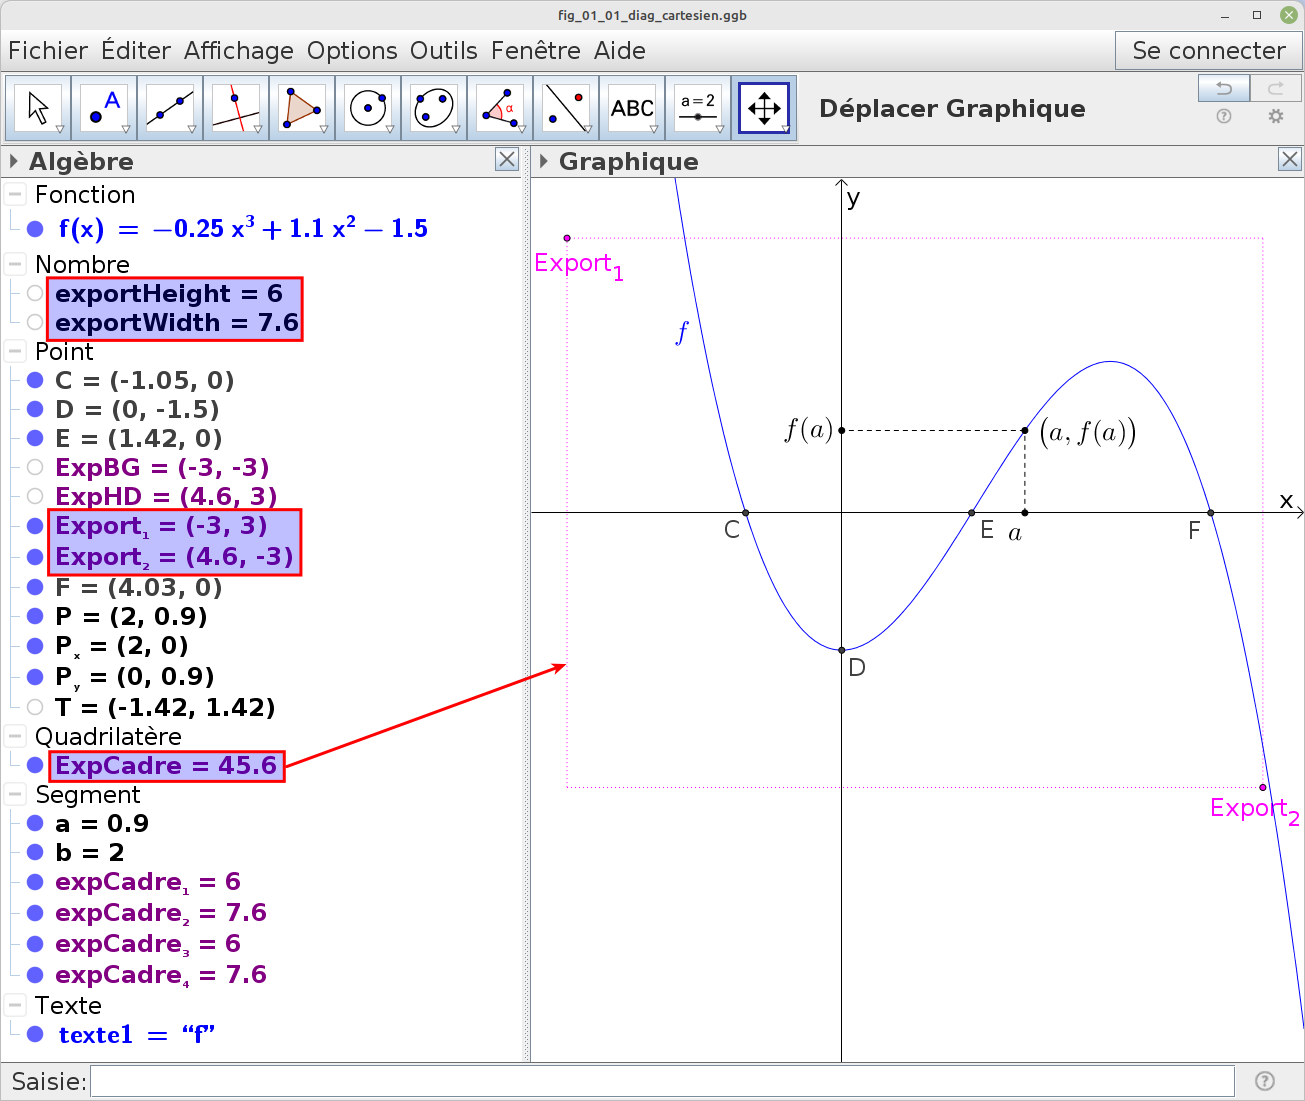
\includegraphics[width=.8\linewidth]{captures/interface_geogebra_aux}
	\caption{}
	\label{fig:interface_geogebra_aux}
\end{figure}

Pour régler le cadre d'export, utiliser les paramètres :
\begin{enumerate}
	\item Le nombre \emph{exportWidth} pour sa largeur en centimètres \\
		Dans les supports de maths les largeurs sont toujours de :
		\begin{itemize}
			\item Pour une image seule sur sa ligne : \SI{12}{cm}
			\item Pour une image occupant la moitié de la ligne : \SI{7.6}{cm}
			\item Pour une image occupant un tiers de la ligne : \SI{4.8}{cm}
		\end{itemize}
	\item Le nombre \emph{exportHeight} sa hauteur en centimètres \\
		On adapte à chaque figure à l'œil.		
	\item Le coin en haut à gauche du cadre : \emph{Export\textsubscript{1}} \\
		\attention Les noms Export\textsubscript{1} et Export\textsubscript{2} sont des mots réservés du langage de GeoGebra. \\
		Si on veut exporter une figure en tant qu'image bitmap, il n'y a pas besoin d'ajuster la fenêtre de GeoGebra : il exporte uniquement ce qu'il y a dans le rectangle défini par ces deux points. Dommage : ça ne marche pas avec un export en TikZ\dots
\end{enumerate}





\newpage





\section{Réaliser et exporter la figure}

\begin{enumerate}
	\item Afficher et régler le cadre d'export \emph{ExpCadre}.
	\item Dessiner la figure.
	\item Lorsque tout est prêt, aligner les bords de la fenêtre sur le cadre d'export.
	\item Masquer le cadre d'export et le point \emph{Export\textsubscript{1}}.
	\item Exporter
		\begin{center}
			Fichier \textrightarrow \ Exporter \textrightarrow \ Graphique vers PGF/TikZ ... 
		\end{center}
	\item On peut arrondir les valeurs qui correspondent au bord de la fenêtre pour éviter d'avoir à les changer dans le fichier \incmd{.tex}.
		\begin{figure}[H]
			\centering
			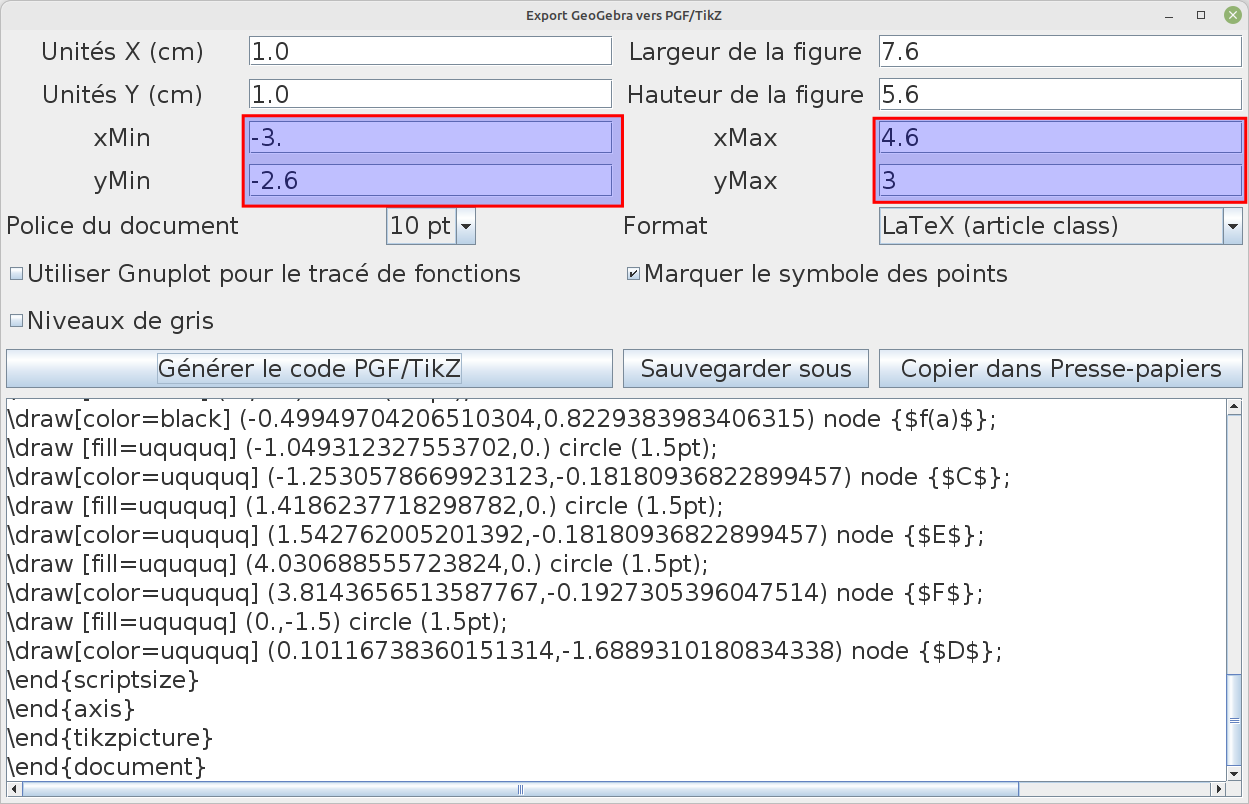
\includegraphics[width=.6\linewidth]{captures/interface_geogebra_export}
			\caption{}
			\label{fig:interface_geogebra_export}
		\end{figure}
\end{enumerate}





\section{Régler la figure dans le fichier .tex}

L'export GeoGebra est tout sauf propre. Il faut le modifier.


\subsection{Positionner les légendes et les textes}

GeoGebra exporte les légendes n'importe où. On doit de toute façon les repositionner à la main.

\subsubsection{Positionnement absolu}

En coordonnées
\begin{itemize}
	\item cartésiennes : \inlatex{\draw[texte] (-0.44,0.9) node {$a$};} pour $x=\SI{-0.44}{cm}$ et $y=\SI{0.9}{cm}$;
	\item polaires : \inlatex{\draw[texte] (45:0.75) node {$a$};} pour $\varphi = \SI{45}{\degree}$ et $\rho = \SI{0.75}{cm}$.
\end{itemize}


\subsubsection{Positionnement relatif}

On peut mémoriser la position d'un point avec \inlatex{coordinate} et le réutiliser ensuite dans un \inlatex{shift}.

Par exemple, pour positionner la légende à \SI{0.6}{em} à la verticale du point $S$ :

\begin{minted}[gobble=1]{latex}
	\draw [point] (-1.5,6.25) coordinate (S) circle (2.0pt);
	\draw[texte,shift=(S)] (90:.6em) node {\scriptsize $S$};
\end{minted}

On peut aussi donner une variation à partir de la position précédente avec \inlatex{+(0cm,1cm)} ou \inlatex{++(2cm,0cm)}. La différence entre les deux est que la première ne change pas le point de référence à partir duquel on ajoute la variation. Avec la deuxième, on ajoute la variation et la nouvelle position ainsi atteinte devient la référence pour de futures positions. Par exemple, pour faire un carré :

\begin{minted}[gobble=1]{latex}
  \begin{minipage}{.25\linewidth}
    \begin{tikzpicture}
      \coordinate (A) at (0,0);
      \draw[trait,epais] (A) -- +(1,0) -- +(1,1) -- +(0,1) -- cycle;
    \end{tikzpicture}
  \end{minipage}
\end{minted}

\begin{minted}[gobble=1]{latex}
  \begin{minipage}{.25\linewidth}
    \begin{tikzpicture}
      \coordinate (A) at (0,0);
      \draw[trait,epais] (A) -- ++(1,0) -- ++(0,1) -- ++(-1,0) -- cycle;
    \end{tikzpicture}
  \end{minipage}
\end{minted}



\subsection{Uniformiser les styles de traits, points\dots}


\subsubsection{Définition des styles}

Les styles graphiques (traits, points, couleurs, flèches\dots) sont définis de manière centralisée dans le document \incmd{styles/preambule_personnalisation.sty}. Extrait :

\begin{minted}{latex}
% ------------------------------------------------------
% Définition des styles les figures tikz
% ------------------------------------------------------
\definecolor{rouge}{rgb}{1,0,0}

\tikzset{rouge/.style={color=rouge}}

\tikzset{trait/.style={draw=black,line width=0.75pt}}
\tikzset{epais/.style={line width=2pt}}
\tikzset{tille/.style={dash pattern=on 2pt off 2pt}}
\end{minted}

Pour utiliser ces styles, on les places entre crochets, séparés par des virgules. Par exemple : 

\begin{minted}[gobble=1]{latex}
	\draw [trait,tille,epais,rouge] (-3.,3.)-- (-3.,-3.);
\end{minted}



\subsubsection{Connecter le fichier .tex aux styles}

Remplacer le préambule : \\

\begin{minipage}{.35\linewidth}
	\begin{minted}[gobble=2]{latex}
		\documentclass[10pt]{article}
		\usepackage[utf8]{inputenc}
		\usepackage{pgfplots}
		\pgfplotsset{compat=1.15}
		\usepackage{mathrsfs}
		\usetikzlibrary{arrows}
		\pagestyle{empty}
		\begin{document}
	\end{minted}
\end{minipage}
{\huge\textrightarrow \quad}
\begin{minipage}{.4\linewidth}
	\begin{minted}[gobble=2]{latex}
		!TeX encoding = UTF-8
		!TeX spellcheck = fr
		!TeX program = xelatex
		\documentclass[11pt]{report}
		\usepackage{../styles/preambule_college}
		\usepackage{../styles/preambule_personnalisation}
		
		\begin{document}
	\end{minted}
\end{minipage}


\subsubsection{Styles de couleur}

L'export de GeoGebra redéfinit les couleurs. On peut supprimer toutes les lignes correspondantes :
\begin{minted}[gobble=1]{latex}
	\definecolor{uququq}{rgb}{0.25098039215686274,0.25098039215686274,0.25098039215686274}
	\definecolor{qqqqff}{rgb}{0.,0.,1.}
	\definecolor{ffqqff}{rgb}{1.,0.,1.}
\end{minted}


\subsubsection{Styles de flèches, axes, échelle}

On peut supprimer les définitions correspondantes de GeoGebra en enlevant le crochet et tout ce qu'il contient dans
\begin{minted}[gobble=2]{latex}
	\begin{tikzpicture}[line cap=round,line join=round,>=triangle 45,x=1.0cm,y=1.0cm]
\end{minted}

\hspace*{4cm}
{\huge\textrightarrow \quad}
\begin{minipage}{.4\linewidth}
	\begin{minted}[gobble=2]{latex}
		\begin{tikzpicture}
	\end{minted}
\end{minipage}

\remarque*{
	Selon la version de GeoGebra utilisée, les axes, leur numérotation et le quadrillage sont générés de diverses manière. Actuellement, un environnemnet \inlatex{axis} du package \href{http://mirrors.ctan.org/graphics/pgf/contrib/pgfplots/doc/pgfplots.pdf}{pgfplots} est utilisé.
}


\subsubsection{Styles de point}

\begin{minted}[gobble=1]{latex}
	\draw [fill=black] (2.,0.9) circle (1.5pt);
\end{minted}

\hspace*{4cm}
{\huge\textrightarrow \quad}
\begin{minipage}{.4\linewidth}
	\begin{minted}[gobble=2]{latex}
		\draw [point] (2.,0.9) circle (1.5pt);
	\end{minted}
\end{minipage}


\subsubsection{Styles de trait}

\begin{minted}[gobble=1]{latex}
	\draw [line width=0.8pt,dotted,color=ffqqff] (-3.,3.)-- (-3.,-3.);
\end{minted}

\hspace*{4cm}
{\huge\textrightarrow \quad}
\begin{minipage}{.4\linewidth}
	\begin{minted}[gobble=2]{latex}
		\draw [trait,tille,bleu] (-3.,3.)-- (-3.,-3.);
	\end{minted}
\end{minipage}


\subsubsection{Styles de texte}

\begin{minted}[gobble=1]{latex}
	\draw[color=black] (1.859475975098335,-0.3893116243683739) node {$a$};
\end{minted}

\hspace*{4cm}
{\huge\textrightarrow \quad}
\begin{minipage}{.4\linewidth}
	\begin{minted}[gobble=2]{latex}
		\draw[texte] (-0.44,0.9) node {$a$};
	\end{minted}
\end{minipage}





\section{Et finalement...}

Finalement, il ne reste "plus" qu'à importer la figure du fichier .tikz (voir figure \ref{fig:fig_01_01_diag_cartesien})

\begin{figure}[H]
	\Centering
	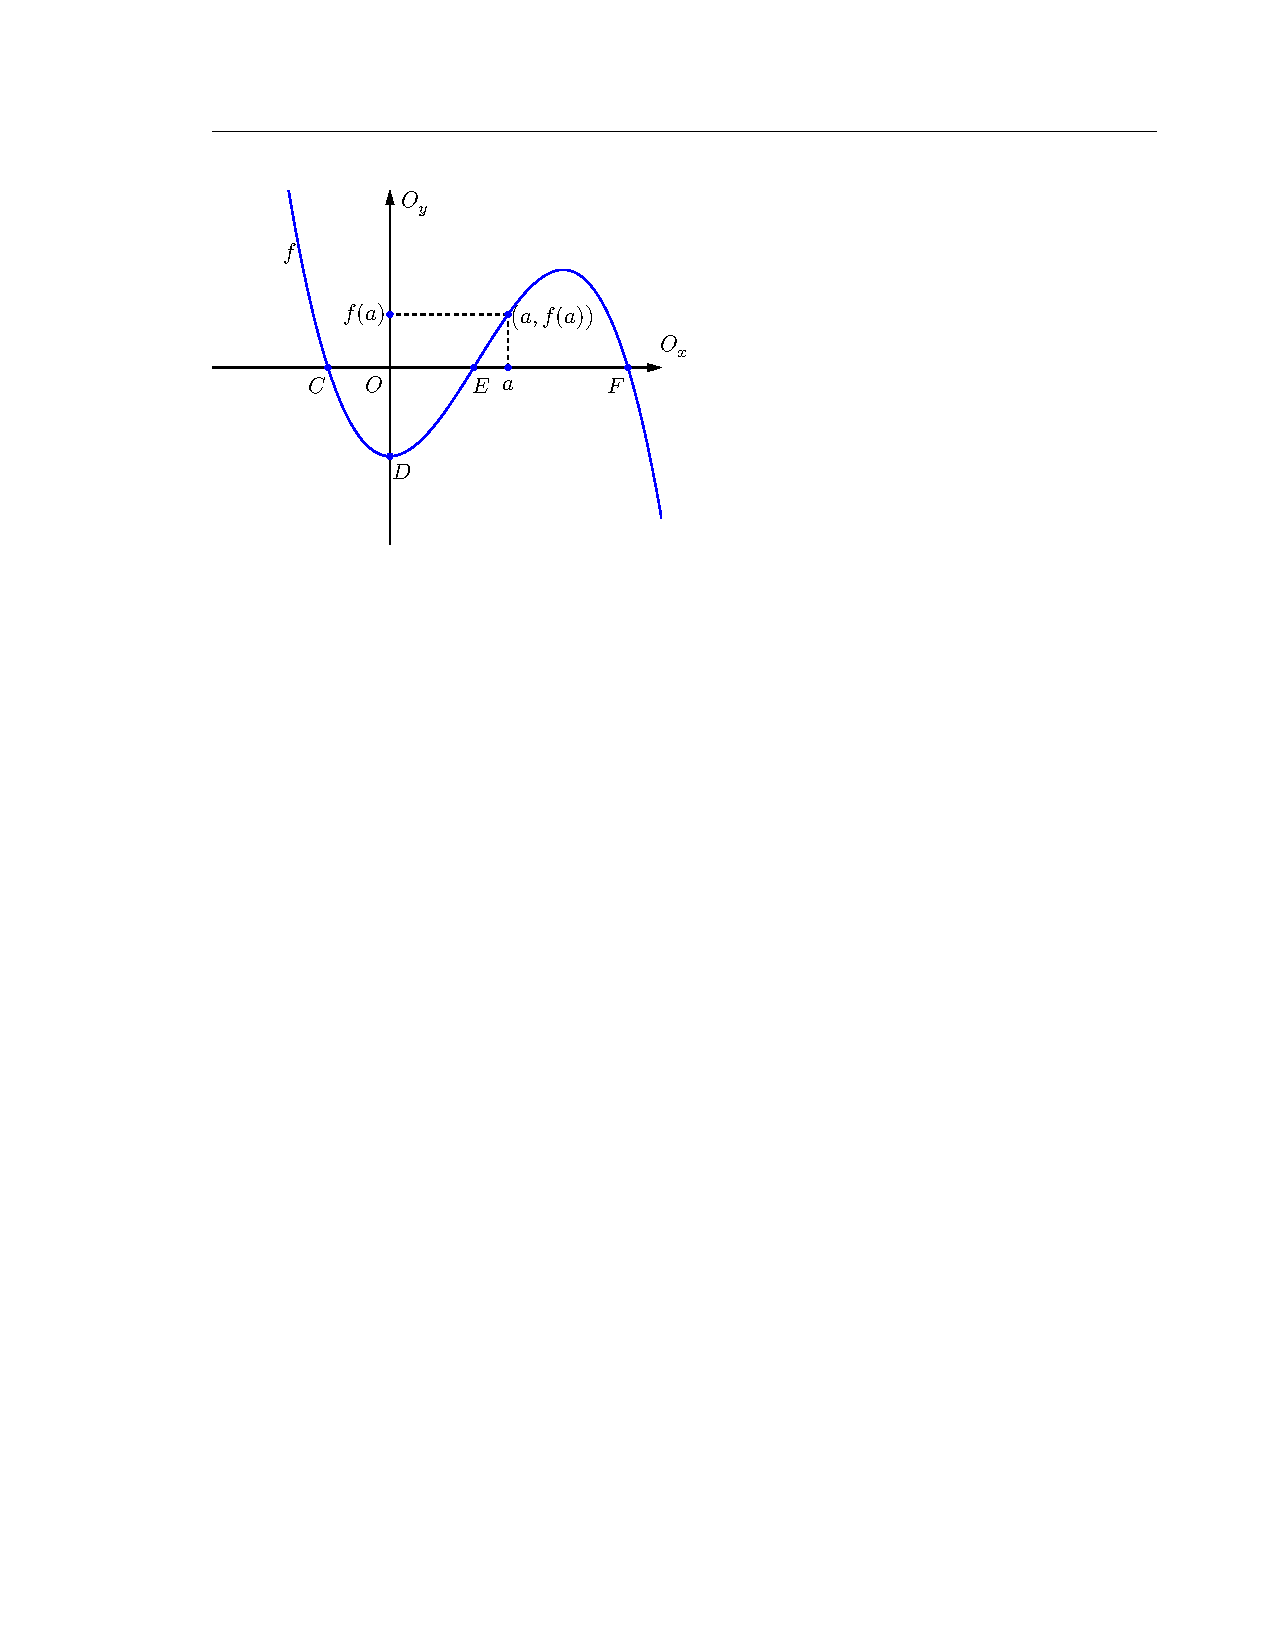
\includegraphics{figures/fig_01_01_diag_cartesien.tikz}
	\caption{}
	\label{fig:fig_01_01_diag_cartesien}
\end{figure}





\end{document}